\section{Used Models and Images}
\label{sec:data}
% vortrainierte Neural Networks erklären/erwähnen
% alle basieren auf der Image Database "ImageNet"
For the upcoming experiments in section \ref{sec:evaluation} we need to decide which network model we use and what images are feasible as source or \emph{guide image}.
As classification network we chose to use \emph{ResNet} because it is the current state of the art providing the lowest error rate and hence performs best.\cite{cnnComparison}

By analyzing various existing \emph{dreamed images}, we came to the conclusion that images with a lot of varying objects offering different features might lead to interesting results.
Hence we were looking for images containing: Landscape with varying vegetation, Houses, water because it offers a lot of noise to act upon, clouds because of the real-life relatability mentioned in section \ref{sec:visual-aspects}.
To find images usable for this purpose we took to \emph{Flickr} because it allows to search for images licensed under the \emph{creative commons}.
There we found three images of interest. Figure \ref{fig:imgbeestemarkt} is an image of the Beestemarkt in Leiden and offers three of the wanted features: water, clouds and buildings.
In addition to that a few people are also in the picture that might turn into interesting things.
The second image visible in figure \ref{fig:imgfield} is a closeup of some vegetation on a field offering a lot of small distinctive features. It contains two of the features we are looking for namely a landscape with varying vegetation and clouds. It is also advantageous that the grass land in the background is made up of different colors ranging from green to yellow to almost brownish.
The third image, portrayed in figure \ref{fig:imglandscape} is similar to the second one but offers different wanted features because it also includes small houses, a properly visible start of a forest, and also there are not many distinctive clouds but just one big grey shadow.


\begin{figure}[H]
	\minipage{0.32\textwidth}
	\centering
	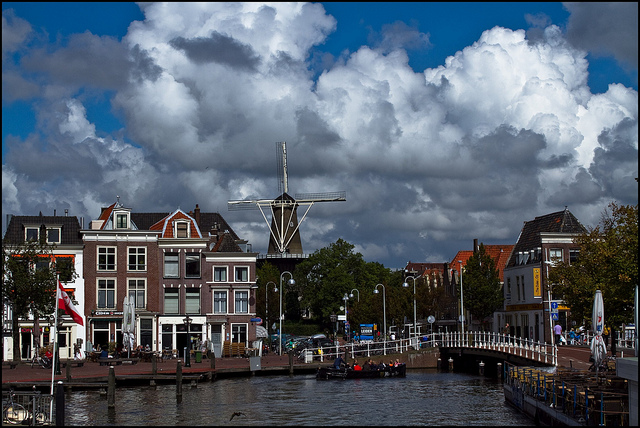
\includegraphics[width=0.5\linewidth]{img/beestemarkt.jpg}
	\caption{Source image displaying the Beestemarkt in Leiden\cite{imgbeestemarkt}.}
	\label{fig:imgbeestemarkt}
	\endminipage\hfill
	\minipage{0.32\textwidth}
	\centering
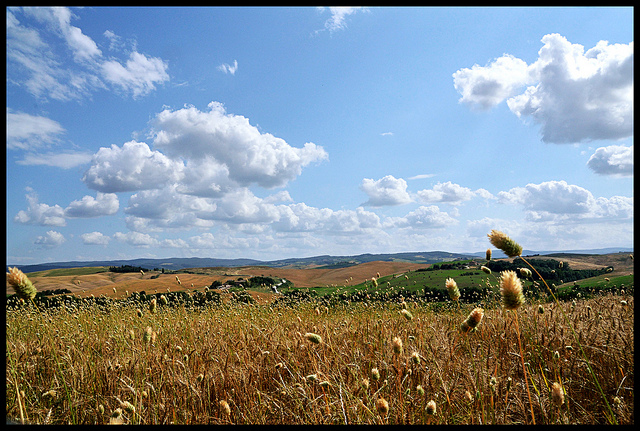
\includegraphics[width=0.5\linewidth]{img/field.jpg}
\caption{Source image portraying a field with mountains in the background\cite{imgfield}.}
\label{fig:imgfield}
\endminipage\hfill
\minipage{0.32\textwidth}
\centering
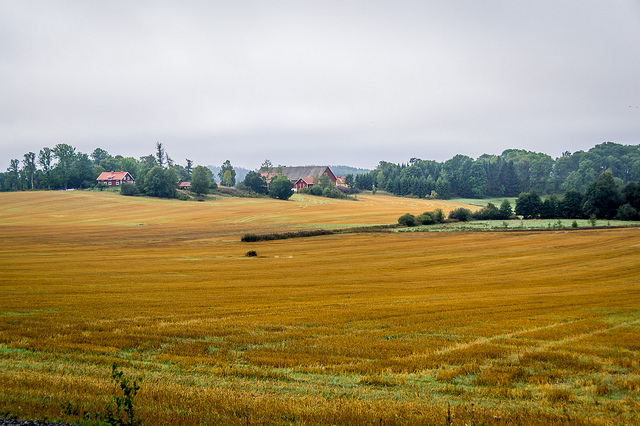
\includegraphics[width=0.5\linewidth]{img/landscape.jpg}
\caption{Source image portraying a landscape with a small houses and trees\cite{imglandscape}.}
\label{fig:imglandscape}
\endminipage\hfill
\end{figure}